\chapter{Tail loss?}

\section{Introduction}


Chordates are composed of three subphyla\textemdash vertebra, tunicata and cephalochordata\textemdash that all share several characteristics, the notochord being the key characteristic, which is indicative of the phyla name. The tail development of larvacean (Oikopleura) and several species of ascidians, tunicates have been studied \cite{jeffery_factors_1992,nakatani_mutations_1999,kugler_evolutionary_2011}. Larvacean form tailed larvae with a hollow dorsal notochord and keep there tail throughout their adult life stage, ascidians do the same before undergoing the process of metamorphosis. A typical ascidian larvae tail forms through the convergence, intercalation and extension of the notochord \cite{swalla_mechanisms_1993}. When fully formed the ascidian notochord contains 40 cells, flanked by three rows of muscle. The ancestral notochord or notochord-like structure is believed to have been muscle based, this is perhaps the reason behind the tail formation being tied to both notochord and muscles \cite{lauri_development_2014}. This is not a far fetched idea seeing that the primary and secondary notochord and muscle lineage are derived from the same blastomere, and the ascidian tail needs both the notochord and differentiated muscle to form a larval tail \cite{nishida_cell_1987,di_gregorio_tail_2002}.

Of the \mytilde3000 species of ascidians less than 20 have been identified as undergoing tail-loss. Although each case of tail loss has happened independently, many of the ascidian that have undergone tail-loss tend to be Molgulide species \cite{berrill_studies_1931,huber_evolution_2000}. Although the mechanism behind tail-loss differs by species, a common characteristic is the lack of a notochord that intercalates and extends. \textit{M. bleizi} notochord cells converge to the midline, and began to extend, however, cells never properly intercalated and the tail formation stop before it is fully formed \cite{jeffery_evolution_1999}. In \textit{M. bleizi} there is an early down-regulation of \textit{bra}\textemdash a key notochord inducer\textemdash and muscle actin (\textit{MbMA}) has become pseudo genes.   

The same process was observed in \textit{M. occulta}, muscle actin becoming pseudo genes, however, the mutations were not the same \cite{swalla_novel_1993}. \textit{M. occulta} and \textit{M. oculata} are two closely related species, who in their adult form are virtually identical, with the exception of a white pigment spot between the two siphons of the tailed species, \textit{M. oculata}. During development the species are indistinguishable up to the gastrula stage. It is at late gastrula when the notochord and muscle cells begin to move posteriorly. There are several steps that take place to form the notochord and tail; first the notochord cells move mediolaterally to the midline, next the cells polarize and intercalate, changing their shape and extending posteriorly \cite{keller_mechanisms_2000, jiang_ascidian_2005,stemple_structure_2005}. This process is known as convergence and extension. 
genes necessary for tail formation that is missing from M. occulta has been found in other ascidians, for instance, macho-1 has been found the tail-less M. tectiformis. 
----
With advances in high throughput sequencing technologies, gene expression of M. occulta, M. oculata, and hybrid species can be analyzed \cite{gyoja_analysis_2007,pickrell_variation_2010}. The transcriptomes of three different developmental stages of M. occulta, M. oculata, and hybrids have been sequenced at Michigan State University. The three transcriptomes were used to identify the presence or absence of known notochord genes downstream of bra using C. intestinalis data from the NCBI database. BLAST searches were with known notochord genes, and several of them were selected for further analysis. FGF9/16/20, prickle (pk), and several other downstream brachyury factors?noto6, leprecan, merlin, and noto17?were analyzed for presence, temporal and spatial expression using in situ hybridizations. In addition to focusing on the notochord genes an EdgeR differential expression analysis was done to identify other genes that are involved in tail development.

Simple body plan with a small number of cells \cite{satoh_ascidian_2001,satoh_genome_2002}, rapid embryo development.

Induced at the 32 cell stage by \textit{FGF9/16/20}
muscle and notochord come from the same cell lineage.
Hybrids are tails are resorted in embryos that contain p58, which stains in the muscle 
It is thought that the early form of the notochord where not cartilage based but were made of muscle.   
----
\section{Methods}
\subsection{Sample collection, sequencing and assembly}
DNA was extracted from the gonads of an individual adult specimen for \textit{M. occidentalis}, \textit{M. occulta}, and \textit{M. oculata}. Paired in jumping libraries were collected for each sample ranging from \mytilde300bp to \mytilde950bp. Further details about extraction methods and libraries can be found in Stolfi et al., \cite{stolfi_divergent_2014}. RNA was extracted from all three \textit{Molgula} species using the methods discussed in Lowe et al., \cite{}. RNA for the gastrula (3hpf), neurla (4hpf) and mid-tailbud (6hpf) stages were extracted for both \textit{M. occulta} and \textit{M. ocultat}, with a replicate for the gastrula and another early-tailbud stage sequenced from \textit{M. occulta}. Stages 7hpf, 16hpf, and 20hpf were taken for \textit{M. occidentalis} to gain a broad scope of expression. Sequencing for \textit{M. occulta} and \textit{M. oculata} RNA were conducted at the Michigan State University, well all other sequencing was done at New York University. All libraries were paired-end, with 75 base pair (bp) reads for the sequencing done at MSU and 100 bp reads for the NYU sequencing. 

Genome assemblies were conducted using 3-pass digital normalization \cite{brown_reference-free_2012} and assembled using Velvet\cite{zerbino_velvet:_2008}. Other assemblers were tested, however, Velvet produced the best results by having the least fragmented assemblies. Assemblies initially done with 21 $\leq$ k $\geq$ 71, for intervals of 10. Assemblies were selected for the highest N50, than assemblies were repeated for a 6 around the selected k. A k of 31, 49, and 37 were select for \textit{M. occulta}, \textit{M. oculata}, and \textit{M. occidentalis}, respectively. 

Both de novo and reference based assembly were used when creating gene models. Reads were mapped to their respective genomes using bowtie2 and tophat to identify genes and alternative splicing variants \cite{langmead_fast_2012,trapnell_differential_2012}. The accepted.bam files were then sorted and indexed using samtools \cite{li_sequence_2009}. The sorted bam files where then processed using cufflinks and cuff merge to generated consenus gtf annotation files. The digitally normalized trinity de novo assembled transcripts from Lowe et al., were aligned to their respective genomes using BLAT \cite{haas_novo_2013}. The cufflinks/cuffmerged gtf files were then covered into bed file and the read mapped annotation and de novo assembled aligned annotation files were merged using gimme (https://github.com/likit/gimme). Gimme joins gene models using a graph based method to develop more complete transcripts. The gimme gene models were then converted to gff format using the script bed2gff in the gimme utils folder in order to extract the transcripts from the genome in a multi pasta file. Transcripts were then extracted using ``gffread -w transcripts.fa -g /path/to/genome.fa transcripts.gtf'' which is included in the cufflinks package. The extracted transcripts were then partitioned into transcript families using khmer partitioning tool and steps found in the eel-pond protocol \cite{}. \textit{Ciona intestinalis} was used as a reference, and the sequences were retrieved as discussed in Chapter 3. 

\subsection{Gene counts and differential expression analysis}
Reads were mapped to transcripts from the gimme gene modules for their respective species. Hybrid reads are mapped onto the \textit{M. occulta} and \textit{M. oculata} transcripts as well, seeing that they are F1 hybrids and should contain an allele from each parent. Read counts were generated using express \cite{}. Express gives the option of ``Total counts'' and ``Effective counts'', which reports the number of reads mapped per transcript and the normalized counts based on transcript length, respectively. Because EdgeR insist on unnormalized reads, ``Total counts'' were used. A replicate was only provided for one of the samples, 3hpf, because of this various dispersion calculation methods were used. the one replicate was used to calculated statistics, in addition to 5hpf being treated as a replicate for 6hpf. These time points represent what would be early and mid-tail bud stages in the urodele ascidian. 

Notochord genes have been identified using subtractive hybridization, mircoarrays and 

\section{Results}
\subsection{\textit{M. occulta} and \textit{M. oculata} have strong overlap in gene presence}
\textit{C. intestinalis} is the closest ascidian species with a well annotated gene, because of these reason it was used to annotate the genomes of both \textit{M. occulta} and \textit{M. oculata}. 

-----
\subsection{Notochord gene network}

The gene modules for \textit{M. occulta} and \textit{M. oculata} produced 42,365 and 407,75 sequences total, respectively. Reciprocal best hit (RBH) blast with an e-value of 1e-3, were done with the \textit{M. occulta} and \textit{M. oculata} transcriptomes against \textit{C. intestinalis} for the annotation of each species.  We are aware this is a low threshold for homologue, however, seeing that on a large-scale, information for these species are not known and we wanted to gain any possible insight go the composition of the genes present in each species. \textit{M. occulta} 8627 annotated / ortho 22700 annotated / homolog \textit{M. oculata} 8,677 annotated were orthologs, 22,583 were annotated homologs. \textit{M. occulta} and \textit{M. oculata} have a high overlap in number of translated transcripts that showed any level of homology with \textit{C. intestinalis} proteins from the NCBI database. Of the 16,414  proteins \textit{M. occulta} had BLAST hits for 83.6\% and 86.5\% had hits in \textit{M. oculata}. \textit{M. occulta} had an additional 453 transcripts that were not found in M. oculata and M. oculata had an additional 921 transcripts that did not have hits in M. occulta, overlapping by 97\%. Next, we examined genes associated with notochord development in C. intestinalis to better analyze the molecular development of the tail.  Seventy-two genes identified as being involved in notochord development (Kugler et al 2008; Hotta et al 2000; Kugler et al. 2011; Jose?-Edwards 2011) were BLAST against each species. Four genes?not1, not4, not5, and snail?were not found in either of the species. This could have been due to true absence or sequence divergence in the transcripts. The remaining 68 genes were shared by both species with the exception of col5a, which was missing from M. occulta. Several genes found in the Ciona notochord GRN were not discovered in either M. occulta or M. oculata. Noto1, noto5, noto14, noto16, and ... were all missing from the transcriptomes of M. occulta and M. oculata. Additionally Kihf5 was not found in M. oculata but showed homology in M. occulta. M. occulta did not have 3 genes that were found in M. oculata, netrin, noto9 and something. 

    Several studies have been done to identity genes involve with tail formation and notochord development, by identifying downstream genes of \textit{bra}\textemdash a key notochord inducer \cite{hotta_temporal_1999,hotta_characterization_2000,hotta_brachyury-downstream_2007,kugler_evolutionary_2008,kugler_evolutionary_2011}. From these studies many potential notochord genes were identified, we compiled a list of x genes and identified there presence or absence within the genomes and transcriptomes of both \textit{M. occulta} and \textit{M. oculata}. Of the x genes x were missing from the transcriptomes of both species, those genes were, \textit{cofilin}, \textit{entactin} (\textit{nidogen-2-like}), \textit{fibrinogen-like protein} (\textit{FGL}), \textit{fibronectin}, \textit{multidom}, \textit{myomegalin}, \textit{noto1}, \textit{noto5}, \textit{noto14}, \textit{noto16}, and \textit{tropomyosin}. Of the remaining genes without orthologus sequences were \textit{netrin}, and \textit{noto9} in \textit{M. occulta} and \textit{Klf15} in \textit{M. oculata}. \textit{Netrin} is involved with the motor neuron, which \textit{M. occulta} does not never seeing that it no longer has the ability to swim. \textit{Klf15} was identified to be in the notochord, but there is currently no know function associated with the gene. This shows a strong overlap in the number of notochord associated genes present in both species.


\begin{figure}[tbp]
\centering
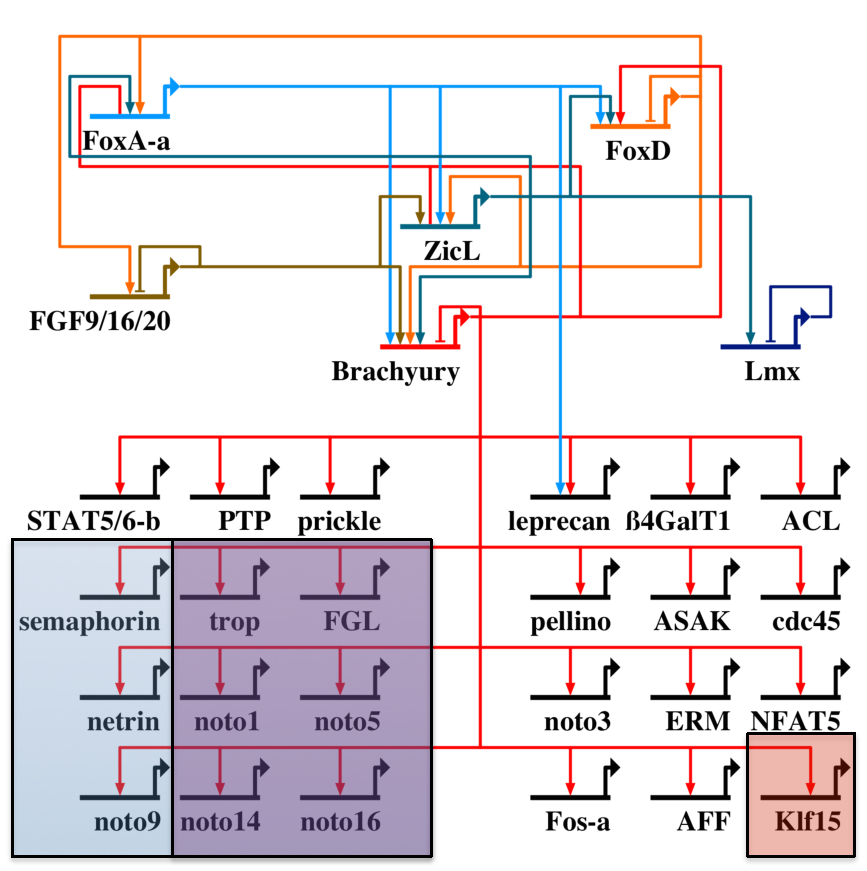
\includegraphics[scale=0.55]{figures/bra_grn.pdf}
\caption{\textbf{Hox cluster for \textit{Hox 10, 12-13} in \textit{M. occulta}, \textit{M. oculata} and \textit{M. occidentalis}} }
\label{fig:bra_grn}
\end{figure}

\begin{figure}[tbp]
\centering
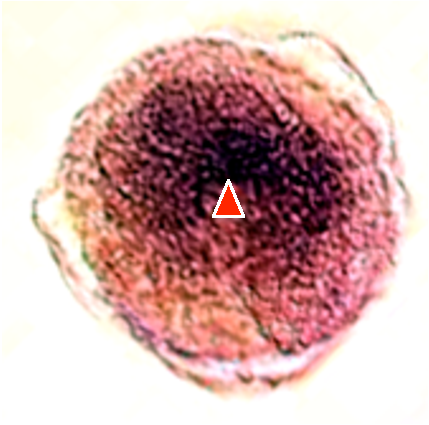
\includegraphics[scale=0.55]{figures/prickle.pdf}
\caption{\textbf{Hox cluster for \textit{Hox 10, 12-13} in \textit{M. occulta}, \textit{M. oculata} and \textit{M. occidentalis}} }
\label{fig:prickle}
\end{figure}



\subsection{Differential expression between neurala and tailbud appears to be key factor is tail development} 

The down regulation of \textit{manx}was shown to be one of the causes behind the tail loss  in \textit{M. occulta}. Three stages\textemdash gastrula, neurula, and tailbud\textemdash were sequenced across \textit{M. occulta}, \textit{M. oculata} and their hybrid. 
during gastrula to neurula 118 up, 63 down and 20285 no significance, 1 noto up 
during gastrula to neurula 260 up, 8 down and 20198 no significance,
during gastrula to neurula 20 up, 93 down and 20353 no significance



during gastrula to neurula 1182 up, 602 down and 18682 no significance, 9 noto up, 1 down. upreg overlap with hyb 349, down 7, up in 
during gastrula to neurula 0 up, 3 down and 20463 no significance
during gastrula to neurula 1277 up, 133 down and 19056 no significance, 7 noto up, 



\textit{M. occulta} and \textit{M. oculata} Gene expression at the gastrula stage does not show a great deal of fold-change between M. occulta, M. oculata and the hybrid. The majority of the genes had a fold-change of less than 5 fold, and most of the genes clustered inside of that 5-fold window (Figure 3a).  The fact that the majority of the genes do not show significant fold-change is not surprising because M. occulta and M. oculata are very similar at this stage of development (Swalla and Jeffery 1990).  When comparing each species to the hybrid, most of the genes clustered within a 5-fold-change window. 
During neurulation M. occulta versus M. oculata differential expression pattern is similar to gastrula stage, clustering within a 5 fold-change window. However, there is a drastic different in the fact that ~300 of the genes have a 10 fold-change in expression (Figure 3d).  The change in expression between the two species mirrors what was observed in morphological studies (Swalla and Jeffery 1990). M. occulta has normal urodele?tailed?development up to gastrula and begins to diverge at neurulation. Of the genes that were higher expressed in M. oculata compared to M. occulta, those same genes were higher expressed in hybrids versus M. occulta. Those genes do not show significant differential expression when comparing M. oculata to hybrid. There are ~20 transcripts that show a 10 fold-change increase in expression in hybrid compared to M. oculata.

\begin{sidewaysfigure}[!ht]
	\subfloat[\label{subfig-1:mocc3v4}]{%
	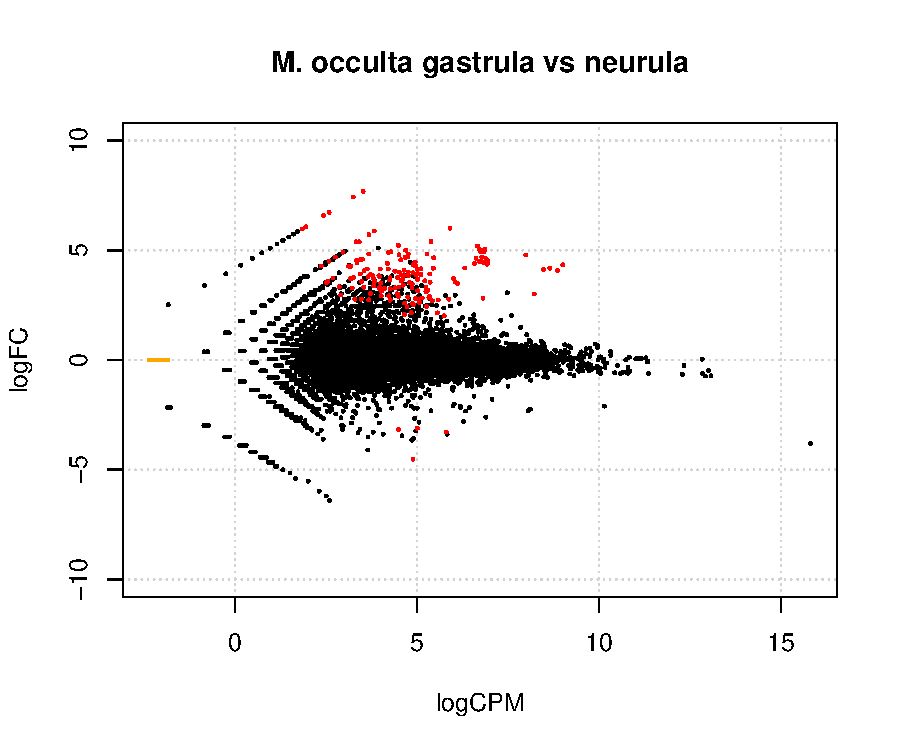
\includegraphics[scale=0.5]{figures/mocc3v4_graph.pdf}
	}
	\subfloat[\label{subfig-2:mocu3v4}]{%
	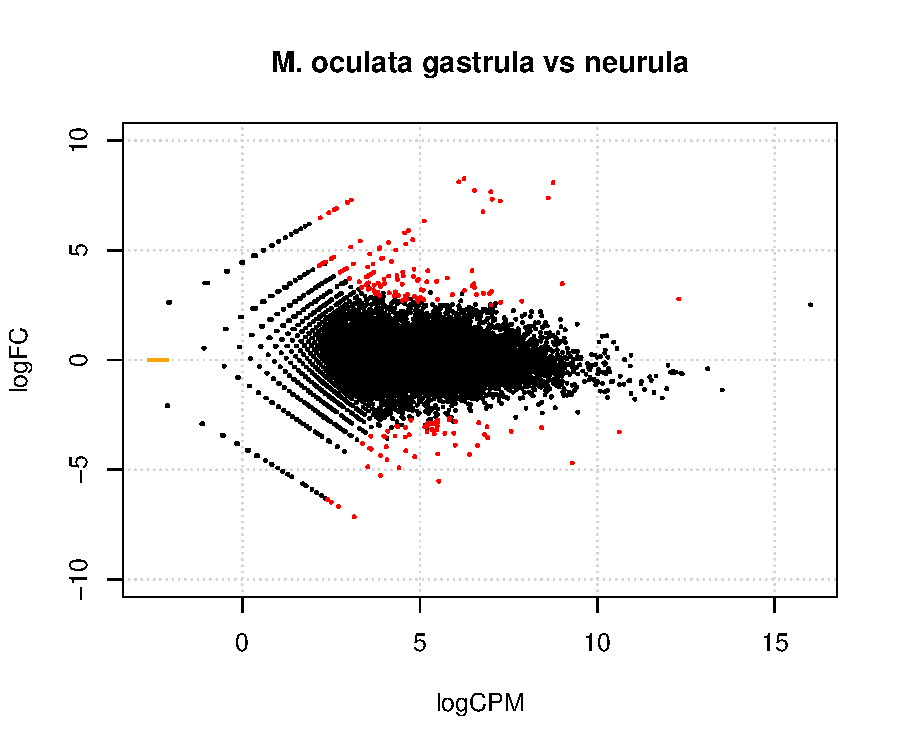
\includegraphics[scale=0.5]{figures/mocu3v4_graph.pdf}
	}
	\subfloat[\label{subfig:hyb3v4}]{%
	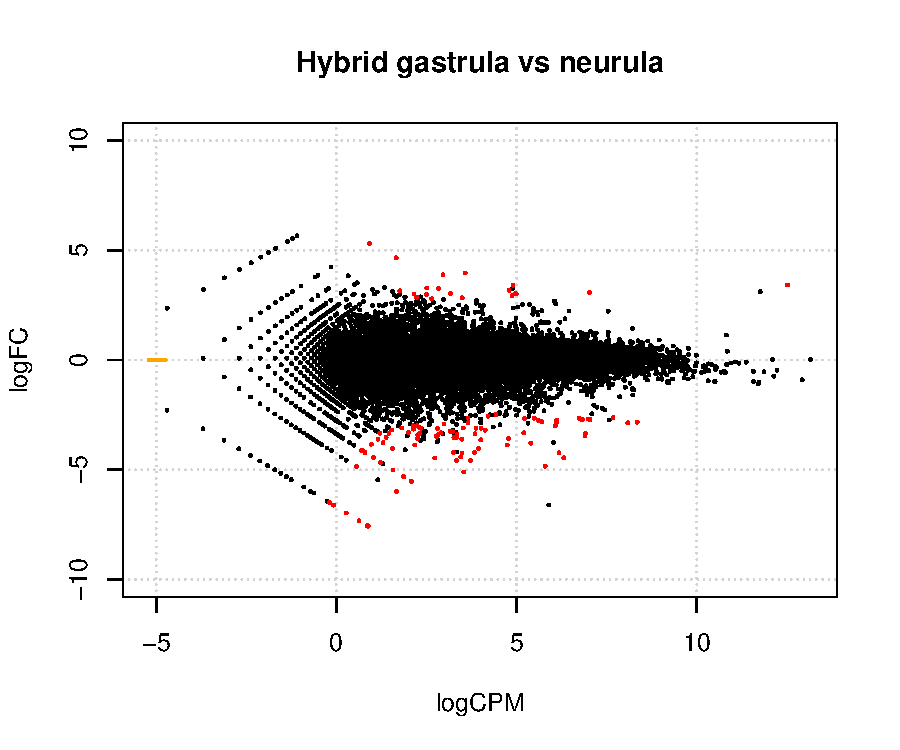
\includegraphics[scale=0.5]{figures/hyb3v4_graph.pdf}
	}
	\hfill
	\subfloat[\label{subfig:mocc4v6}]{%
	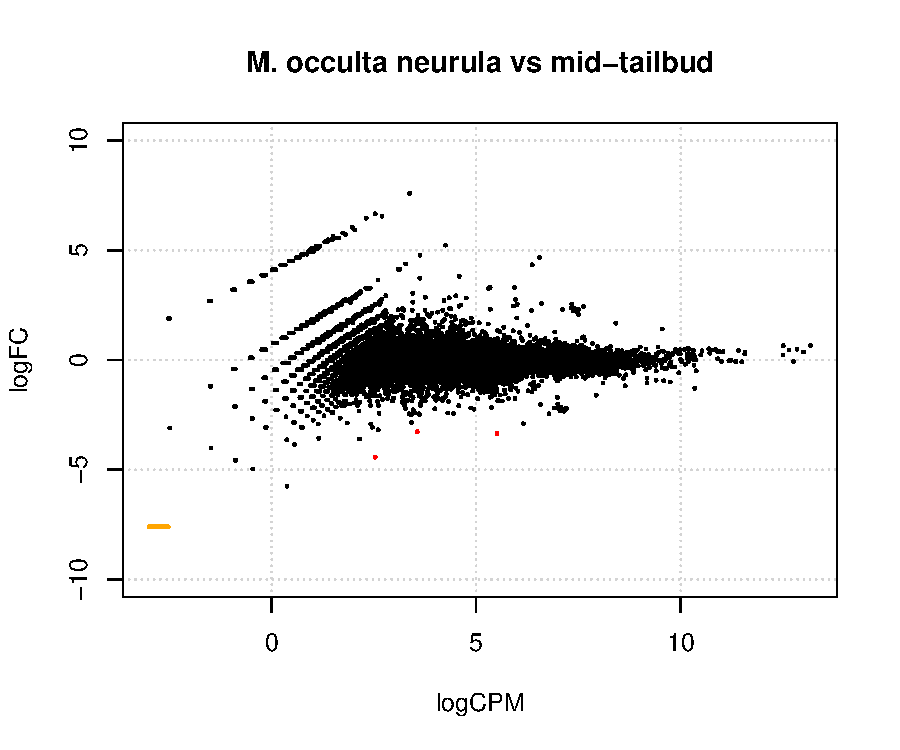
\includegraphics[scale=0.5]{figures/mocc4v6_graph.pdf}
	}
	\subfloat[\label{subfig:mocu4v6}]{%
	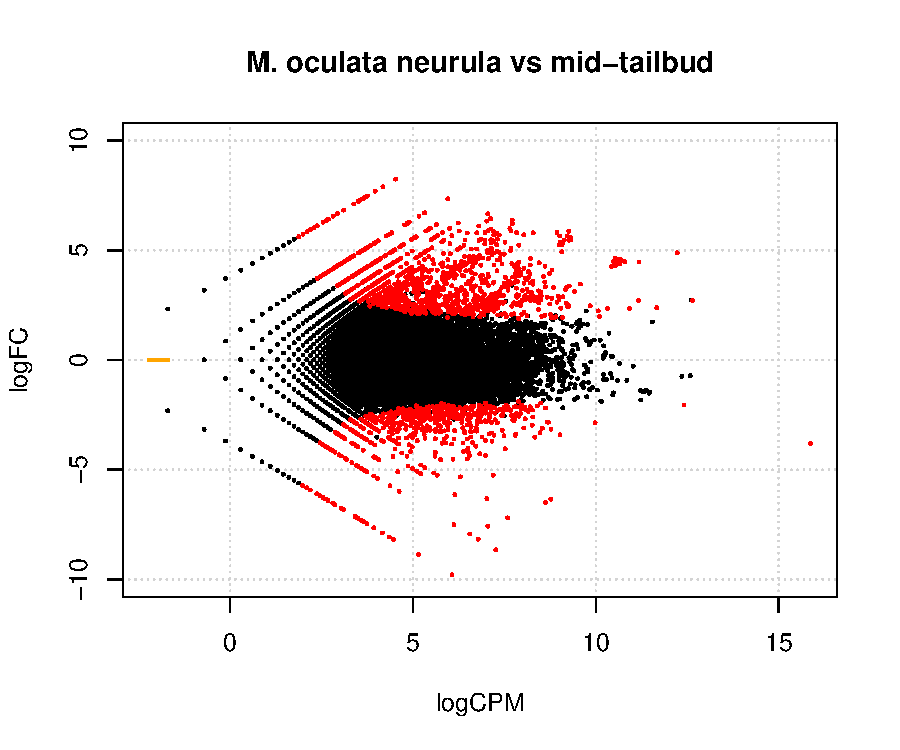
\includegraphics[scale=0.5]{figures/mocu4v6_graph.pdf}
	}
	\subfloat[\label{subfig:hyb4v6}]{%
	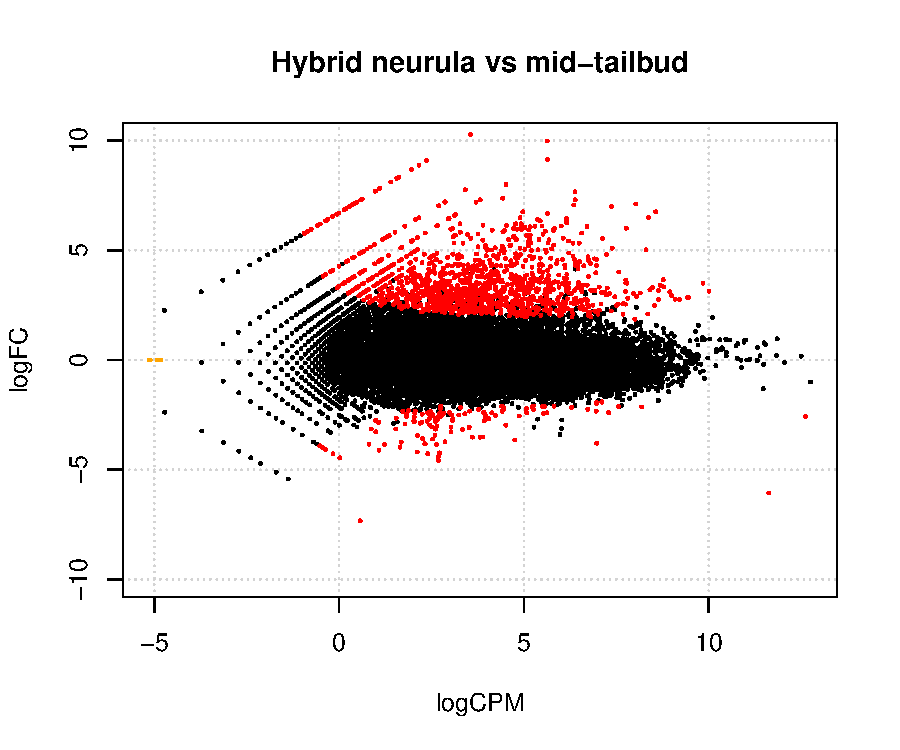
\includegraphics[scale=0.5]{figures/hyb4v6_graph.pdf}
	}
	\caption{\textbf{Differential expression of homologous transcripts.} The k-mer distribution is shown for each assembler and assembly condition, diginorm (DN) and unnormalized reads. The k-mer distribution is the coverage of a given k-mer verses how many k-mers of that coverage is incorporated in the respective assemblies. Both Oases and Trinity assemblies are shown for ~\ref{fig:figure_2_Mocc_dist} \textit{M. occulta} k-mer distribution and  ~\ref{fig:figure_2_Mocu_dist} \textit{M. oculata} k-mer distributions. Trinity had a higher k-mer distribution for both species, reflective of the inclusion of more low abundance reads into the Trinity assemblies.}
	\label{fig:de_plots}
\end{sidewaysfigure}
